\section{Introduction}
Machine Learning (ML), particularly Deep Learning, has significantly advanced the MIR field by enabling automatic feature learning, improving classification and analysis tasks, and facilitating novel applications like music generation and source separation. Adopting musically motivated neural network architectures \cite{musicmotivCNN} blends musical concepts and perceptual approaches and use this knowledge to analyze and understand music in a way that goes beyond traditional music analysis techniques. 

\section{Artificial Neural Networks (ANNs)}
A neural network, formally known as an artificial neural network (ANN), is a computational model inspired by the structure and functionality of biological neural networks. It is a mathematical framework designed to process information and perform tasks like pattern recognition, classification, and regression by mimicking how biological neurons and synapses operate. ANNs comprise interconnected layers of artificial neurons or nodes, each performing a mathematical transformation on the input data to generate an output. The connections between these neurons, often called "weights," are adjusted during learning to optimize the network's performance on a given task.

\subsection{About ANNs}
The concept of neural networks can be traced back to the early 20th century, with the pioneering work of Warren McCulloch and Walter Pitts in 1943. They proposed a mathematical model of a neuron known as the McCulloch-Pitts neuron, which provided a foundation for future research in artificial intelligence. However, Frank Rosenblatt's invention of the perceptron in 1957 marked the beginning of modern neural networks. The perceptron is a single-layer neural network capable of learning linearly separable patterns.

%Single neuron
\begin{SCfigure}[2\sidecaptionrelwidth][h]
	\centering
	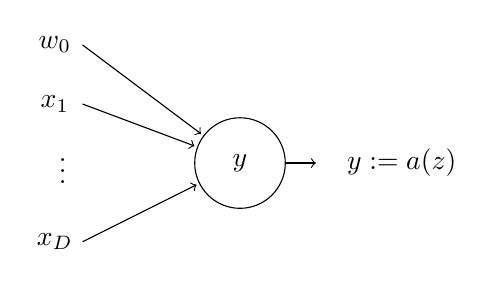
\begin{tikzpicture}[shorten >=1pt,->]
		\tikzstyle{unit}=[draw,shape=circle,minimum size=1.15cm]
 
		\node[unit](p) at (2,1){$y$};
		\node(dots) at (-0.25,1){\vdots};
 
		\draw (0,2.5) node[xshift=-10]{$w_0$} -- (p);
		\draw (0,1.75) node[xshift=-10]{$x_1$} --(p);
		\draw (0,0) node[xshift=-10]{$x_D$} -- (p);
		\draw (p) -- (3,1) node[xshift=30]{$y := a(z)$};
	\end{tikzpicture}
	\caption[Single processing units and its components.]{\small{Single processing unit and its components. The activation function is denoted by $a$ and applied to the actual input $z$ of the unit to form its output $y = a(z)$. $x_1, \ldots, x_D$ represent input from other units within the network; $w_0$ is called bias and represents an external input to the unit. The propagation rule maps all inputs onto the actual input $z$.}}
	\label{fig:processing-unit}
\end{SCfigure}

In a more technical description, an ANN consists of an input layer, one or more hidden layers, and an output layer. Each neuron in a layer receives input from the previous layer and computes an output value using an activation function. Some standard activation functions include the sigmoid, hyperbolic tangent (tanh), and rectified linear unit (ReLU). The output of the last layer represents the prediction or classification result.

%NN
\input{figures/neural networks/Network_graph}

%Multi-layer_NN
\begin{figure}[ht]
	\centering
	% NEURAL NETWORK with coefficients, shifted
\begin{tikzpicture}[x=2.2cm,y=1.4cm]
  \message{^^JNeural network, shifted}
  \readlist\Nnod{4,5,5,5,3} % array of number of nodes per layer
  \readlist\Nstr{n,m,m,m,k} % array of string number of nodes per layer
  \readlist\Cstr{\strut x,a^{(\prev)},a^{(\prev)},a^{(\prev)},y} % array of coefficient symbol per layer
  \def\yshift{0.5} % shift last node for dots
  
  \message{^^J  Layer}
  \foreachitem \N \in \Nnod{ % loop over layers
    \def\lay{\Ncnt} % alias of index of current layer
    \pgfmathsetmacro\prev{int(\Ncnt-1)} % number of previous layer
    \message{\lay,}
    \foreach \i [evaluate={\c=int(\i==\N); \y=\N/2-\i-\c*\yshift;
                 \index=(\i<\N?int(\i):"\Nstr[\lay]");
                 \x=\lay; \n=\nstyle;}] in {1,...,\N}{ % loop over nodes
      % NODES
      \node[node \n] (N\lay-\i) at (\x,\y) {$\Cstr[\lay]_{\index}$};
      
      % CONNECTIONS
      \ifnum\lay>1 % connect to previous layer
        \foreach \j in {1,...,\Nnod[\prev]}{ % loop over nodes in previous layer
          \draw[connect,white,line width=1.2] (N\prev-\j) -- (N\lay-\i);
          \draw[connect] (N\prev-\j) -- (N\lay-\i);
          %\draw[connect] (N\prev-\j.0) -- (N\lay-\i.180); % connect to left
        }
      \fi % else: nothing to connect first layer
      
    }
    \path (N\lay-\N) --++ (0,1+\yshift) node[midway,scale=1.5] {$\vdots$};
  }
  
  % LABELS
  \node[above=0.8,align=center,mygreen!60!black] at (N1-1.90) {input\\[-0.2em]layer};
  \node[above=0.5,align=center,myblue!60!black] at (N3-1.90) {hidden layers};
  \node[above=1.3,align=center,myred!60!black] at (N\Nnodlen-1.90) {output\\[-0.2em]layer};
  
\end{tikzpicture}
	\caption[Network graph for perceptron.]{\small{Network graph of a perceptron with $D$ input units and $C$ output units. The $l^{\text{th}}$ hidden layer contains $m^{(l)}$ hidden units. Each neuron in a layer receives input from the previous layer and computes an output value using an activation function. The output of the last layer represents the prediction or classification result.
}}
	\label{fig: multilayer color perceptron}
\end{figure}

\section{Deep Learning (DL)}

%Backpropagation
\input{figures/neural networks/Back_propagation}

\subsection{Convolutional Neural Network (CNN)}

A Convolutional Neural Network (CNN) is a deep-learning neural network. The architecture of a CNN is composed of several layers, including:

\begin{itemize}

\item \textbf{Convolutional layers:} These layers apply a convolution operation to the input data. The raw audio data can be either a 1D signal or transformed into a spectrogram or a Mel-spectrogram representation, which can be considered an image-like 2D representation of the audio data. The convolutional layers are designed to effectively learn local patterns and features in the audio data \footnote{For a visual explanation of convolution, see this video: \url{https://youtu.be/KuXjwB4LzSA}}.

\textbf{1D Convolution Example:} Given a 1D input signal $I = [i_1, i_2, ..., i_n]$ and a filter (or kernel) $K = [k_1, k_2, ..., k_m]$, the convolution operation is defined as $(I * K)j = \sum{u=1}^{m} I_{j-u+1} K_u$, where $j$ ranges from $1$ to $n-m+1$, and $I * K$ represents the resulting feature vector after applying the convolution. The objective of the 1D convolution operation is to slide the filter over the input signal and compute the element-wise product and sum for each local region, effectively learning and detecting local patterns in the input data.

\item \textbf{Pooling layers:} These layers downsample the data, reducing the spatial or temporal dimensions of the input while retaining important information. A joint pooling operation is the max-pooling, which can be defined as follows: given an input matrix $I$ and a pooling window of size $m \times n$, the max-pooling operation selects the maximum value within each non-overlapping $m \times n$ region of the input matrix. This operation effectively reduces the input's dimensions while retaining the most essential information in each region.
\vspace*{3mm}

\item \textbf{Fully connected layers:} These layers connect every neuron in one layer to every neuron in another, allowing the network to learn non-linear combinations of the features learned in the previous layers. Mathematically, a fully connected layer can be represented as $Y = XW + b$, where $X$ is the input matrix, $W$ is the weight matrix, $b$ is the bias vector, and $Y$ is the output matrix. The nonlinearity is introduced through the activation function, which is applied element-wise to the output matrix, such as $Y' = f(Y)$, where $f$ represents the activation function and $Y'$ is the transformed output matrix.
\vspace*{3mm}

\item \textbf{Output layer:} The output layer produces the final predictions of the network.

\end{itemize}

Compared to a traditional neural network, CNNs are more computationally efficient and have less number of parameters to train. This makes them more feasible for large-scale datasets and real-world problems.

On top of that, one of the main advantages of using CNNs for audio analysis is that they can automatically and adaptively learn temporal hierarchies of features from audio data, which traditional audio processing methods may not do effectively. 

%CNN
\input{figures/neural networks/CNN_diagram}

%Single CNN
\input{figures/neural networks/Single_CNN}

%Single pooling layer
\input{figures/neural networks/Single_Pooling_Layer}

\newpage


